\documentclass[12pt]{article}

\usepackage{styles/log-style}

\begin{document}
\begin{titlepage}
\begin{center}
\bfseries

{\Large Московский Авиационный Институт\\ (национальный исследовательский университет)}

\vspace{36pt}

\large Институт информационных технологий и прикладной математики

\vspace{36pt}

\large Кафедра вычислительной математики и программирования

\vspace{48pt}

Журнал по исследовательской практике (индивидуальный план)

\end{center}

\vspace{120pt}

\begin{flushleft}
\begin{tabular}{|r|l|}
\hline
Студенты & Группа \\
\hline
Артемьев Дмитрий Иванович & М8О-406Б-18 \\
\hline
Белоусов Егор Владимирович & М8О-207Б-20 \\
\hline
Инютин Максим Андреевич & М8О-307Б-19 \\
\hline
Команда: & MAI \#2 Artemiev, Belousov, Inyutin \\
\hline
\end{tabular}
\end{flushleft}

\vspace*{\fill}

\begin{center}
\bfseries
Москва, \the\year
\end{center}
\end{titlepage}

\pagebreak

\subsection*{Сводная таблица за осень \the\year}
\resizebox{\columnwidth}{!}{
\begin{tabular}{|c|c|c|c|c|c|}
\hline
Дата & Название & Время & Место проведения & Решенные задачи & Дорешанные задачи \\
\hline
12.09.2021 & Grand Prix of Dolgoprudny & 11:00-16:00 & Дистанционно & A, B & C\\
\hline
19.09.2021 & Grand Prix of IMO & 11:00-16:00 & Дистанционно & A, B & C\\
\hline
26.09.2021 & Grand Prix of XiAn & 11:00-16:00 & Дистанционно & A, B & C\\
\hline
10.10.2021 & XXII Открытая Всесибирская олимпиада & 10:00-15:00 & Дистанционно & A, B & C\\
\hline
24.10.2021 & Grand Prix of Korea & 11:00-16:00 & Дистанционно & A, B & C\\
\hline
07.11.2021 & Grand Prix of Siberia & 11:00-16:00 & Дистанционно & A, B & C\\
\hline
14.11.2021 & Grand Prix of EDG & 11:00-16:00 & Дистанционно & A, B & C\\
\hline
21.11.2021 & RuCode 4.0 Div A-B Champoinship & 11:00-16:00 & Дистанционно & A, B & C\\
\hline
17.10.2021 & ICPC training MAI 21-22 & 11:00-16:00 & Дистанционно & A, B & C\\
\hline
28.11.2021 & Grand Prix of Southern Europe & 11:00-16:00 & Дистанционно & A, B & C\\
\hline
05.12.2021 & Grand Prix of Poland & 11:00-16:00 & Дистанционно & A, B & C\\
\hline
12.12.2021 & Grand Prix of Nanjing & 11:00-16:00 & Дистанционно & A, B & C\\
\hline
19.12.2021 & Moscow Regional Contest & 11:00-16:00 & Дистанционно & A, B & C\\
\hline
\end{tabular}
}

\subsection*{Явка на контесты}
\resizebox{\columnwidth}{!}{
\begin{tabular}{|c|c|c|}
\hline
Дата & Название & Присутствующие \\
\hline
12.09.2021 & Grand Prix of Dolgoprudny & Артемьев, Белоусов, Инютин \\
\hline
19.09.2021 & Grand Prix of IMO & Артемьев, Белоусов, Инютин \\
\hline
26.09.2021 & Grand Prix of XiAn & Артемьев, Белоусов, Инютин \\
\hline
10.10.2021 & XXII Открытая Всесибирская олимпиада & Артемьев, Белоусов, Инютин \\
\hline
24.10.2021 & Grand Prix of Korea & Артемьев, Белоусов, Инютин \\
\hline
07.11.2021 & Grand Prix of Siberia & Артемьев, Белоусов, Инютин \\
\hline
14.11.2021 & Grand Prix of EDG & Артемьев, Белоусов, Инютин \\
\hline
21.11.2021 & RuCode 4.0 Div A-B Champoinship & Артемьев, Белоусов, Инютин \\
\hline
17.10.2021 & ICPC training MAI 21-22 & Артемьев, Белоусов, Инютин \\
\hline
28.11.2021 & Grand Prix of Southern Europe & Артемьев, Белоусов, Инютин \\
\hline
05.12.2021 & Grand Prix of Poland & Артемьев, Белоусов, Инютин \\
\hline
12.12.2021 & Grand Prix of Nanjing & Артемьев, Белоусов, Инютин \\
\hline
19.12.2021 & Moscow Regional Contest & Артемьев, Белоусов, Инютин \\
\hline
\end{tabular}
}

\pagebreak

\includepdf[pages=10, scale=0.75, pagecommand=\subsection*{Grand Prix of Dolgoprudny 12.09.2021}]{statements/210830.pdf}
\subsubsection*{Идея}
Тут вы описываете идею решения, оцениваете сложность...

Например, сложность жадного алгоритма $O(n \cdot \log{n})$, а перебор $O(2 ^ {n} \cdot n ^ 2)$.
\subsubsection*{Исходный код}
\lstinputlisting{src/gp_dolgop_g.cpp}
\subsubsection*{Положение команды}
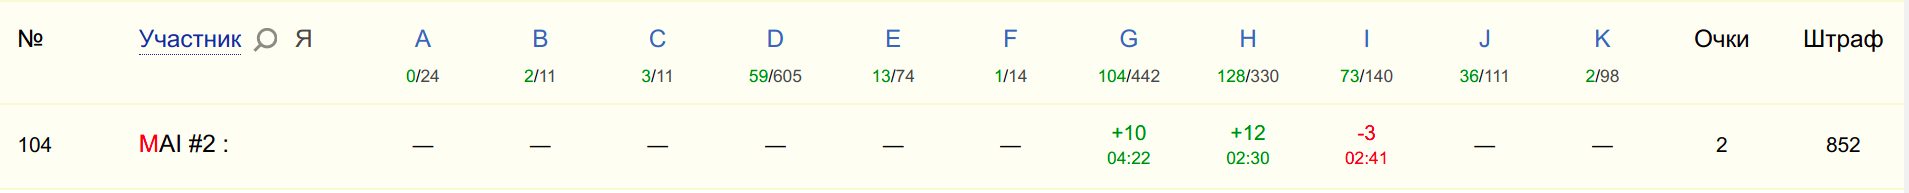
\includegraphics[scale=0.25]{images/gp_dolgop.png}\newline\noindent

\end{document}
